\documentclass{article}

\usepackage{fancyhdr}
\usepackage{extramarks}
\usepackage{amsmath}
\usepackage{amsthm}
\usepackage{amsfonts}
\usepackage{tikz}
\usepackage{algorithm}
\usepackage{mathtools}
\usepackage{algpseudocode}
\usepackage{booktabs}
\usepackage{multirow}
\usepackage{rotating}
\usepackage{adjustbox}
\usepackage{hyperref}


\usetikzlibrary{automata,positioning}

%
% Basic Document Settings
%

\topmargin=-0.45in
\evensidemargin=0in
\oddsidemargin=0in
\textwidth=6.5in
\textheight=9.0in
\headsep=0.25in


\linespread{1.1}

\pagestyle{fancy}
\lhead{\hmwkAuthorName}
\chead{\hmwkClass\ (\hmwkClassInstructor\ \hmwkClassTime): \hmwkTitle}
\rhead{\firstxmark}
\lfoot{\lastxmark}
\cfoot{\thepage}

\renewcommand\headrulewidth{0.4pt}
\renewcommand\footrulewidth{0.4pt}

\setlength\parindent{0pt}

%
% Create Problem Sections
%

\newcommand{\enterProblemHeader}[1]{
    \nobreak\extramarks{}{Problem \arabic{#1} continued on next page\ldots}\nobreak{}
    \nobreak\extramarks{Problem \arabic{#1} (continued)}{Problem \arabic{#1} continued on next page\ldots}\nobreak{}
}

\newcommand{\exitProblemHeader}[1]{
    \nobreak\extramarks{Problem \arabic{#1} (continued)}{Problem \arabic{#1} continued on next page\ldots}\nobreak{}
    \stepcounter{#1}
    \nobreak\extramarks{Problem \arabic{#1}}{}\nobreak{}
}

\setcounter{secnumdepth}{0}
\newcounter{partCounter}
\newcounter{homeworkProblemCounter}
\setcounter{homeworkProblemCounter}{1}
\nobreak\extramarks{Problem \arabic{homeworkProblemCounter}}{}\nobreak{}

\newenvironment{homeworkProblem}[1][-1]{
    \ifnum#1>0
        \setcounter{homeworkProblemCounter}{#1}
    \fi
    \section{Problem \arabic{homeworkProblemCounter}}
    \setcounter{partCounter}{1}
    \enterProblemHeader{homeworkProblemCounter}
}{
    \exitProblemHeader{homeworkProblemCounter}
}

\newcommand{\solutionIntro}[5]{
\thispagestyle{plain} 
\newpage
\setcounter{page}{1}
\noindent
\begin{center}
\framebox{ \vbox{ \hbox to 6.28in
{\bf ME598: Deep Reinforcement Learning \hfill #4}
\vspace{4mm}
\hbox to 6.28in
{\hspace{2.5in}\large\mbox{#5}}
\vspace{4mm}
\hbox to 6.28in
{#1 \hfill {\it Professor \textit{#2}}}
}}
\end{center}
\markright{#1}
}

\newcommand{\hmwkTitle}{Homework\ \#2}
\newcommand{\hmwkDueDate}{February 12, 2014}
\newcommand{\hmwkClass}{Calculus}
\newcommand{\hmwkClassTime}{Section A}
\newcommand{\hmwkClassInstructor}{Professor Isaac Newton}
\newcommand{\hmwkAuthorName}{Josh Davis}

%
% Title Page
%

\title{
    \vspace{2in}
    \textmd{\textbf{\hmwkClass:\ \hmwkTitle}}\\
    \normalsize\vspace{0.1in}\small{Due\ on\ \hmwkDueDate\ at 3:10pm}\\
    \vspace{0.1in}\large{\textit{\hmwkClassInstructor\ \hmwkClassTime}}
    \vspace{3in}
}

\author{\textbf{\hmwkAuthorName}}
\date{}

\renewcommand{\part}[1]{\textbf{\large Part \Alph{partCounter}}\stepcounter{partCounter}\\}

\newcommand{\solution}{\textbf{Solution: }\\}

\begin{document}

\solutionIntro{Ehsan Saleh}{Matthew West and Timothy Bretl}{2}{Fall 2018}{Project Report}

\pagestyle{myheadings}  % Leave this command alone

\section{Introduction}

Reinforcement Learning can provide policies for controlling robotic movements. Recent progress in robotics devices development \cite{haewon} raised the need for intelligent robot controllers. In this project, we will try to design a robotic controller for a single-foot robot by simulation. The robot was intended to avoid obstacles that come across
while running on a conveyor belt. The reinforcement learning model used for this project was the proximal policy optimization \cite{Schulman2017}.

\section{Implementation Keys and Details}

For the purpose of simulation, we chose to use bullet as the the physics engine, and the pybullet API for creating simulation environments. We will highlight some of the challenging parts of using this physics engine properly:
\begin{itemize}
	\item Enabling self collision including the parent links can make the simulation more realistic. Especially since non-trained agents tend to make the robot hit itself.
	\item Defining the right friction models has high impact on the behavior of contacts. The default contact properties of this engine seem to be slippery. The robot description file can be found in the ``urdf'' folder of the supplementary code and material.
	\item Deactivating the joint motors is also an important step. The joint motors are turned on by default.
\end{itemize}

Furthermore, reward shaping is also a very crucial step for training a successful agent. We will highlight some of the components used for training agents on similar robots.
\begin{itemize}
	\item The simplest reward function maximizes the potential energy of the robot. However, the optimal policy for this reward could make the robot jump too high distances.
	\item To account for the instability of this reward function, we may need to add motor energy consumption cost.
	\item The motor energy consumption may cause the robot to lean on itself for movement or standing, which is inappropriate. Therefore, adding self collision cost would also be appropriate.
	\item Adding other costs such as stall torque cost, or penalizing for the angular displacement may also help stabilize the robot movement.
	\item Colliding with obstacles should also be considered separately for a more significant penalty in order to be avoided properly.
\end{itemize}

\section{Sample Training curves}

In the following figures, you can see the learning curves produced during training the agent.

\begin{figure}[H]
	\centering
	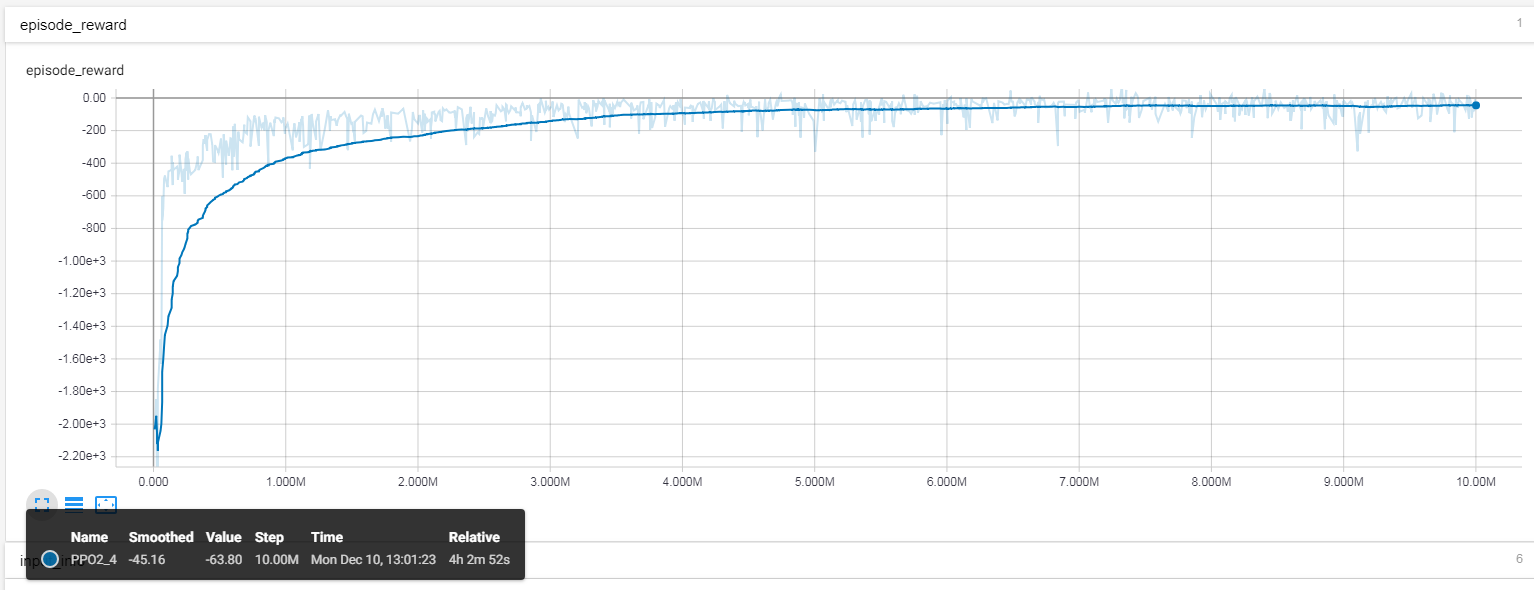
\includegraphics[width=0.8\textwidth]{../trainplots/EpisodeReward}
	\caption{The learning curve for the total episode reward}
\end{figure}
\begin{figure}[H]
	\centering
	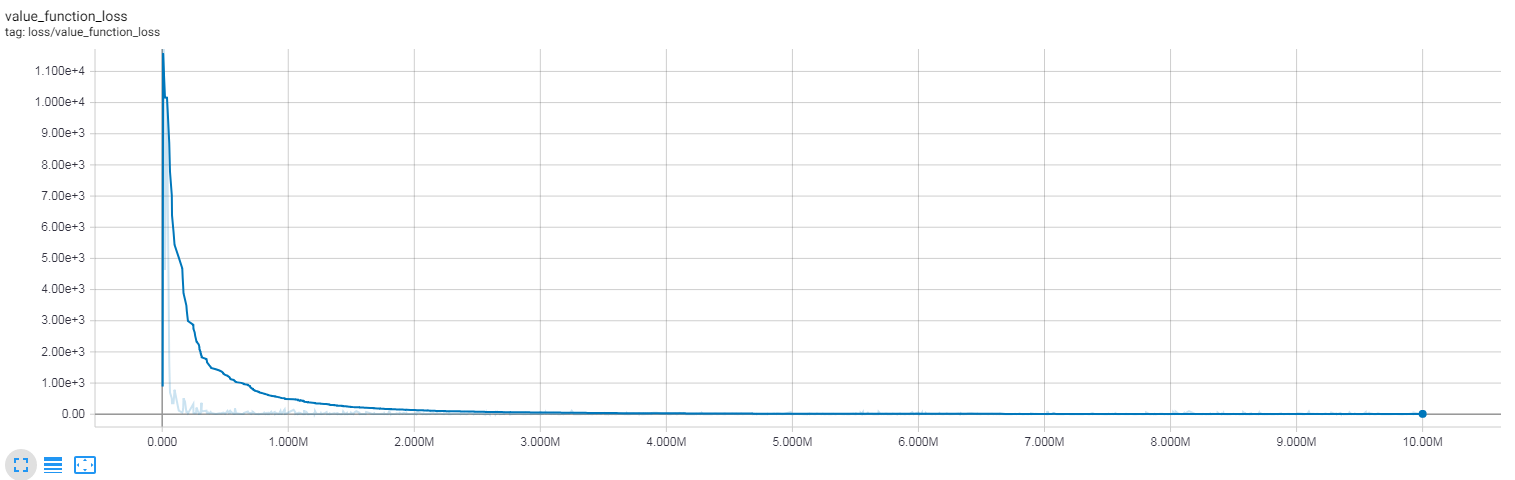
\includegraphics[width=0.8\textwidth]{../trainplots/ValueLoss}
	\caption{The learning curve for the value function loss}
\end{figure}
\begin{figure}[H]
	\centering
	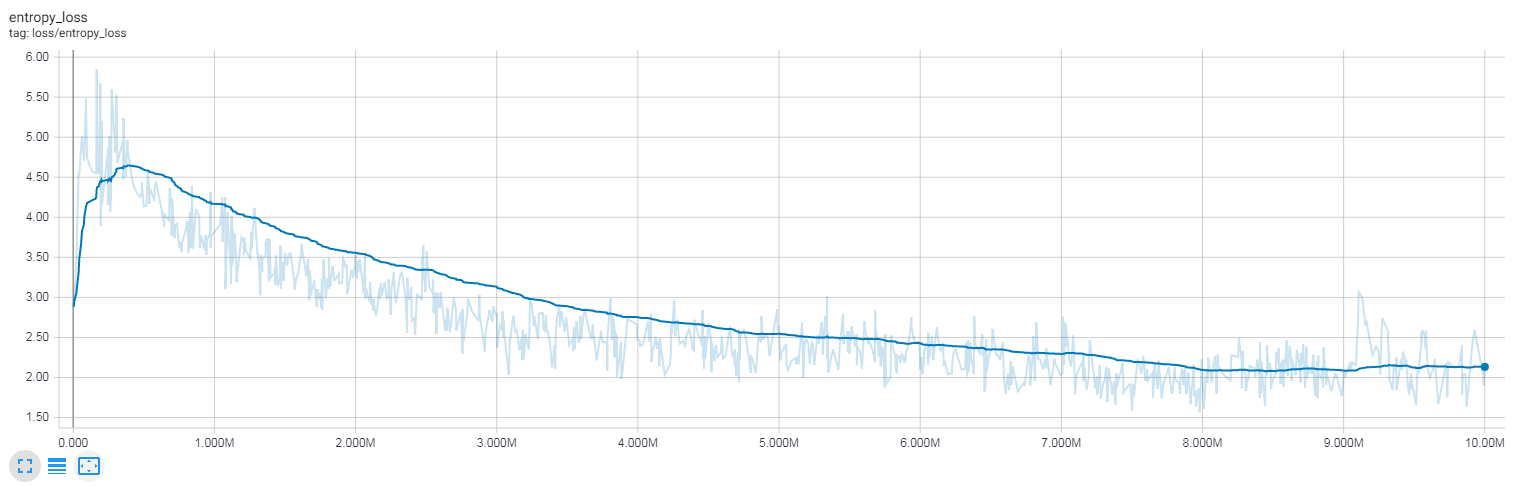
\includegraphics[width=0.8\textwidth]{../trainplots/EntropyLoss}
	\caption{The learning curve for the entropy loss}
\end{figure}

\bibliographystyle{siam}
\bibliography{bib}

\end{document}

